\subsection{Shift register}

\begin{minted}[
   fontsize=\footnotesize,
   linenos,
   breaklines,
]{verilog}
module shift_reg #(
   parameter DataWidth = 4,
   parameter Depth = 3  // FIXME: Depth is actullay hard-coded
)(
   input clk_i,
   input rst_ni,
   input enable_i,
   input  [DataWidth-1:0] d_i,
   output [DataWidth-1:0] reg_0_o,
   output [DataWidth-1:0] reg_1_o,
   output [DataWidth-1:0] reg_2_o
);

reg [DataWidth-1:0] mem_d [0:Depth-1];
reg [DataWidth-1:0] mem_q [0:Depth-1];

// TODO: more flexible
assign reg_0_o = mem_q[0];
assign reg_1_o = mem_q[1];
assign reg_2_o = mem_q[2];

integer i;

always @(posedge clk_i, negedge rst_ni)
   if (!rst_ni)
      for(i = 0; i < Depth; i = i + 1)
         mem_q[i] <= 0;
      // For SystemVerilog, use array assignment pattern with the default keyword:
      // mem_q <= '{default: '0};
   else
      for(i = 0; i < Depth; i = i + 1)
         mem_q[i] <= mem_d[i];

always @(enable_i, mem_q) begin

   // default assignment next state is present state
   for(i = 0; i < Depth; i = i + 1)
      mem_d[i] = mem_q[i];

   if (enable_i) begin
       for(i = Depth - 1; i > 0; i = i - 1)
          mem_d[i] = mem_d[i-1];
       mem_d[0] = d_i;
   end

end

endmodule
\end{minted}

\begin{minted}[
   fontsize=\footnotesize,
   linenos,
   breaklines,
]{verilog}
module shift_reg_tb;

parameter DataWidth = 5;

// Inputs
reg clk;
reg rst_n;
reg enable_i;
reg [DataWidth-1:0] d_i;

// Outputs
wire [DataWidth-1:0] reg_0_o;
wire [DataWidth-1:0] reg_1_o;
wire [DataWidth-1:0] reg_2_o;

shift_reg #(
   .DataWidth(DataWidth)
) DUT (
   .clk_i(clk),
   .rst_ni(rst_n),
   .enable_i(enable_i),
   .d_i(d_i),
   .reg_0_o(reg_0_o),
   .reg_1_o(reg_1_o),
   .reg_2_o(reg_2_o)
);

// Create a 50Mhz clock
always #10 clk = !clk;  // every ten nanoseconds invert

initial begin
   clk = 1'b0;
   rst_n = 1'b0;
   enable_i = 1'b0;
   d_i = 5'd4;
end

initial begin
   #20 rst_n = 1'b1;  // release reset

   // Shift a same value multiple times
   repeat (4) begin
      @(posedge clk);
      enable_i = 1'b1;
      @(posedge clk);
      enable_i = 1'b0;
   end

   // Reset
   @(negedge clk);
   rst_n = 1'b0;
   @(negedge clk);
   rst_n = 1'b1;

   // Shift
   d_i = 5'd7;
   @(posedge clk);
   enable_i = 1'b1;
   @(posedge clk);
   enable_i = 1'b0;

// Finish the Simulation
   #100;
   $finish;
end

endmodule
\end{minted}

\begin{figure}[htbp]
   \centering
   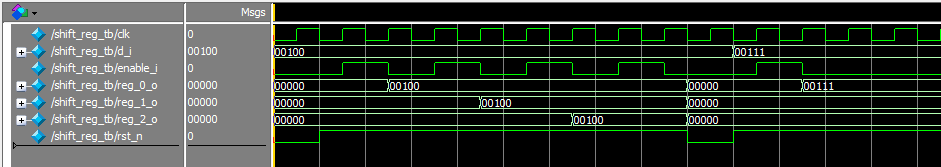
\includegraphics[width=\textwidth]{shift_register_sim.png}
   \caption{Testbench simulation of the shift register module.}
   \label{fig:shift_register_sim}
\end{figure}
